% !TeX root = document.tex
% !TeX encoding = UTF-8 Unicode

\chapter{Switching Rules}%
\label{chp:switching-rules}

This chapter presents two switching rules: the dwell-time, the most employed and
studied of such techniques in literature, and the proposed rule based on the
region of attraction. Other techniques exist, like using robust control to
design a controller that never allows the system to unstabilize; however, they
are more conservative and not viable in many cases.

\section{Dwell-time}%
\label{sec:dwell-time}

As discussed in Section~\ref{sec:switched-systems}, the act of switching can
cause instability, even if all modes are stable. Although it is possible to
verify if the system is stable under arbitrary switching (and therefore to
design controllers to do so), the procedure is not straightforward and
challenging to apply to most real-world situations.

There are, however, other ways of verifying and guaranteeing the stability of
switched systems. The dwell-time is one of such techniques that restricts the
switching signal \(\sigma{}(t)\) to the set
%
\begin{equation}
  \mathcal{D}_{T} := \{\sigma(\cdot):t_{k+1}-t_{k}\ge{}T\},
\end{equation}
%
where \(t_{k}\) and \(t_{k+1}\) are the switching instants, for all
\(k\in{}\mathbb{R}\), which forces the system to remain for \(T\) seconds on a
mode before switching to next one~\parencite{colaneri:dwell}. This is called a
slow switch. The timer is restarted every time the reference changes and
switching is only allowed after \(T\) seconds has passed. For large enough
values of \(T\), this rule guarantees the system's stability.

As the dwell-time certifies stability of the switch, it decouples the switching
logic and the system stability, making it possible to analyse the system
stability for each mode independently. One problem, however, is that computing
the minimum dwell-time is not easy and is the focus of current research. An
easier problem is to find an upper bound for it, which can be done efficiently
using numerical algorithms~\parencite{colaneri:dwell}.

Another technique that uses the concept of dwell-time is the average dwell-time,
where the switching rule \(\sigma\) allows for a fixed number of discontinuities
\(N_{\sigma}(t,\tau)\) for \(t\ge{}\tau{}\ge{}0\) such that the set
\(\mathcal{D}_{T_{D},N_{0}}\) satisfies
%
\begin{equation}
  N_{\sigma}(t,\tau) \le{} N_{0} + \frac{t-\tau}{\tau_{D}},
\end{equation}
%
where \(\tau_{D}\) is the average dwell-time and \(N_{0}\) is the chatter
bound~\parencite{hespanha.morse:stability}. This set is larger than
\(\mathcal{D}_{T}\) and allows for signals with discontinuities separated by at
most \(\tau_{D}\).

To illustrate how the dwell-time works, consider the state-space of a fictional
two-state system shown in Figure~\ref{fig:dt-example}. \(\bullet\) marks the system's
initial state, \(\diamond\) are the waypoints and \(\star\) is the reference. The collored
ellipses are each mode's state's constraints, numbered 1, 2, 3 from left to
right. Since there are three ellipses, we have three modes, meaning three
command governors, controllers and linearized systems. The waypoints are
intermediate references, chosen to allow the system to travel from the current
state (\(\bullet\)) to the reference (\(\star\)) without violating any constraint.

\begin{figure}[ht!]
  \centering
  \begin{tikzpicture}[auto,node distance=3cm,>={Stealth},waypoint/.style={draw,circle,minimum size=1em,inner sep=0pt,outer sep=0pt,thick},state/.style={draw,thick,circle,minimum size=1em,inner sep=0pt,outer sep=0pt},constraint/.style={ellipse,fill opacity=0.7,text opacity=1}]
    \node (x)  [state]                {\(\bullet\)};
    \node (w1) [waypoint,below=of x]  {\(\diamond\)};
    \node (w2) [waypoint,right=of w1] {\(\diamond\)};
    \node (w3) [waypoint,above=of w2] {\(\star\)};

    \begin{scope}[on background layer]
      \node (c1) [constraint,fill=cyan!80,fit=(x) (w1)]    {};
      \node (c2) [constraint,fill=green!80,fit=(w1) (w2)]  {};
      \node (c3) [constraint,fill=orange!80,fit=(w2) (w3)] {};
    \end{scope}

    \draw [->,thick] (x) -- (w1);
    \draw [->,thick] (w1) -- (w2);
    \draw [->,thick] (w2) -- (w3);
  \end{tikzpicture}%
  \caption[Dwell-time illustrative example.]{Dwell-time illustrative example.
    The plane is the phase-plane of a second order system. Each colored region
    represents one mode's contraints, each symbol inside a circle represents a
    point of interest: \(\bullet\) is the initial state, \(\diamond\) are the waypoints and
    \(\star\) the final reference, as set by the operator. The arrows show the path
    the system will take as the supervisor changes the references to the
    waypoints and then to \(\star\).}%
  \label{fig:dt-example}
\end{figure}


Consider that the system is on steady-state at \(\bullet\) when the reference switched
to \(\star\). The supervisor scheme used here is the one given in
Figure~\ref{fig:supervisor-schematic}. The supervisor will receive the new
reference \(r(k)\) and, because the system is currently on mode 1, will set
\(r'(k)\) to the first waypoint's coordinates, since it is not possible to gro
from \(\bullet\) to \(\star\) directly without violating the constraints.

Because a reference change occurred, the supervisor will start a timer, counting
down from the first mode's dwell-time, \(T_{1}\). Even if \(r(k)\) changes
again, \(r'(k)\) will not be changed until this timer expires. This gives the
first mode's controller enough time to converge to the first waypoint,
guaranteeing stability.

Because the waypoint is at mode 1's and mode 2's constraints intersection, the
supervisor is allowed to change the the system to the second mode and change the
reference \(r'(k)\) to the second waypoint's coordinates, as soon as the
dwell-time's timers expire (both changes happen simultaniously). Again, because
the reference changed, a new timer will start, but now counting down from mode
2's dwell-time, \(T_{2}\). The same procedure will be repeated once the system's
state reaches the second waypoint, when \(r'(k)\) will finally be set to
\(r(k)\).

Algorithm~\ref{alg:dwell-time} presents a generalized version of the algorith
described in the given example.

\begin{algorithm}[H]
  \begin{algorithmic}[1]
  \State{}\textbf{Input}: \(\CG{}_i\) \(\leftarrow{}\) current \CG{},~\(\CG{}_j\) \(\leftarrow{}\) target \CG{}.
  \State{}change \(r'(k)\) to next way-point
  \While{dwell-time of \(\CG{}_{i}\) not ellapsed}
    \State{}calculate \(g(k)\)
    \State{}execute controller
  \EndWhile{}
  \State{}change to \(\CG{}_j\)
  \State{}restart algorithm
  \end{algorithmic}
  \caption{dwell-time implementation}%
  \label{alg:dwell-time}
\end{algorithm}

Firstly, \(\CG{}_{i}\) is set to the currently active \CG{} and \(\CG{}_{j}\) to
the next \CG{} in the path (briefly disscussed in
Subsection~\ref{subsec:supervisor}). Then the reference \(r'(k)\) is set to the
next waypoint in the path. The timer is started and the supervisor will wait for
it to ellapse before making any change to the system. While it is not ellapsed,
the active \CG{} and controller will drive the system to the reference
\(r'(k)\). As soon as the time ellapses, the system switches modes, activating
\(\CG{}_{j}\). The procedure is then repeated.

\section{Region of Attraction}%
\label{sec:roa-switching-rule}

The goal of this switching rule is to allow the system to converge faster to the
final reference when going through a path of restricted mode switches. To do so,
it is necessary to:

\begin{enumerate}
  \item guarantee stability after switching modes,
  \item switch modes as soon as possible.
\end{enumerate}

The main contribution of this work is to propose a switching rule based on the
controller's region of attraction yielding a guaranteed stable closed-loop
system. As described in Section~\ref{sec:region-of-attraction}, the controller's
region of attraction is the forward invariant neighbourhood under the flow
generated by a critical point. On a switched system, there is one controller and
linearized system for each mode, therefore there is also one region of
attraction for each mode.

Since the definition of a Region of Attraction undesirably allows the existence
of limit-cycles within the region, we turn to Lyapunov's theorem to further
restrict the region, eliminating them. The set which represents the region of
attraction becomes \textit{contractive}, becoming smaller as the system's state
converges to the critical point. The Lyapunov function is seen as an energy
function, and its value at some point in the state-space is an energy level.
This leads to the so called level sets, which are all points that yield the same
energy level, in Lyapunov's sense.

The level set, denoted \(\mathcal{L}_{V}(P)\), where \(P\) is the matrix used in
the function \(V(x)=x^{\top}Px\), is an estimative of the region of attraction and,
being contractive, implies that, once the system reaches a lower energy level,
in Lyapunov's sense, it can not go to a state with higher energy and can only
stay at the same level if it is zero, which guarantees convergence, as the only
point with zero energy is the origin of the linear system.

The region of attraction is, therefore, a certificate of stability for a system.
However, as stated in Section~\ref{sec:switched-systems}, having stable modes is
not enough to guarantee the stability of the system after switching.
Nonetheless, the following region of attraction based rule guarantees that the
system will remain stable after switching:

\begin{align}
  \sigma_{i} = \begin{cases}
    1 & \textrm{if}~\xi_{i}(k)\in\mathcal{L}_V(P_i) \\
    0 & \textrm{otherwise}
  \end{cases},
\end{align}
%
where \(\xi_{i}(k)\) is the mode's state, and \(\sigma_{i}\) is the switching rule,
meaning that the system can switch to the \(i\)th mode if \(\sigma_{i}=1\). The
switching rule does not force the use of any particular region of attraction
estimation. Any method can be used to estimate the region of attraction, and the
use of Lyapunov's theorem is just an example.

Let us discuss the stability of the system when this rule is used. Suppose a
system with two modes is currently in mode 1, and the supervisor has deemed that
it needs to go mode 2. The switch will only occur when the system's state is
inside the second mode's controller's region of attraction. Because it is inside
the region of attraction, it guarantees that it will converge, and therefore the
switch is stable.

Consider the same scenario, however the system has 10 modes and the switch from
mode 1 to mode 2 follows the path \(1 \rightarrow 3 \rightarrow 8 \rightarrow 2\), meaning that, to go from
\(1\) to \(2\), it first needs to switch to \(3\), then to \(8\) and only then
to \(2\). The worst-case would be if the system is in the middle of the
intersection of all regions of attraction. In this case, the system will
instantly switch modes, going from \(1\) to \(2\) in \(3\) sample times, in the
case of a discrete system. However, since the switch can only happen when the
state is inside the next mode's controller's region of attraction, it will
simply cause the previous scenario to be applied recursivelly, and the system
will remain stable after it reaches the last mode.

In another scenario, the software generating the references for the supervisor
(i.e. generating \(r(k)\)) might malfunction or have a badly defined rule that
will make the reference jump between many values, making the system try to
switch modes seemly randomly. In this case the system will do the switches as
long as it is allowed, but the state will always be inside some controller's
region of attraction. It will then either never converge nor diverge (because of
the ever-changing reference) or enter a state that is only inside one mode's
controller's region of attraction, at which point it will not switch modes
anymore.

The illustrative scenarios show that the state will always be inside some
controller's region of attraction, and therefore it is not possible for the
system to diverge. It can oscilate due to varying references, but that is a case
of malfunction or badly desined referencing system, not normal operation.
Furthermore, when used in conjunction with Command Governors, the reference is
always guaranteed to be inside the region of attraction (since the constraint
region is completely contained inside it), even if the supervisor's reference is
not, eliminating the possible scenario where the system diverges because the
reference is outside the region of attraction, dragging the system out of it.

To illustrate, we will use the same example of Section~\ref{sec:dwell-time}, but
this time applying the region of attraction based rule. A difference, seen in
Figure~\ref{fig:roa-example}, is the presence of the dashed circles,
representing each controller's region of attraction. When the reference
\(r'(k)\) changes to the first waypoint's coordinates, the supervisor will start
checking whether the system's state is inside the region of attraction of the
next mode's controller and, when it enters this region, the controller and
linearized model will be changed to those of the system's mode 2, but the
constraints will still be those of mode 1. We call this a hybrid switch. In
Figure~\ref{fig:roa-example}, the dashed arrows represent a path followed while
in a hybrid mode.

\begin{figure}[ht!]
  \centering
  \captionsetup{justification=centering}
  \begin{tikzpicture}[auto,node distance=3cm,>={Stealth},waypoint/.style={draw,circle,minimum size=1em,inner sep=0pt,outer sep=0pt,thick},state/.style={draw,thick,circle,minimum size=1em,inner sep=0pt,outer sep=0pt},constraint/.style={ellipse,fill opacity=0.7,text opacity=1}]
    \node (x)  [state]                {\(\bullet\)};
    \node (w1) [waypoint,below=of x]  {\(\diamond\)};
    \node (w2) [waypoint,right=of w1] {\(\diamond\)};
    \node (w3) [waypoint,above=of w2] {\(\star\)};

    \begin{pgfonlayer}{background}
      \node (c1) [name path=c1,constraint,fill=cyan!80,fit=(x) (w1)]    {};
      \node (c2) [name path=c2,constraint,fill=green!80,fit=(w1) (w2)]  {};
      \node (c3) [name path=c3,constraint,fill=orange!80,fit=(w2) (w3)] {};
    \end{pgfonlayer}

    \node (roa1) [circle,very thick,draw=cyan!80,dashed,fit=(c1)]   {};
    \node (roa2) [circle,very thick,draw=green!80,dashed,fit=(c2)]  {};
    \node (roa3) [circle,very thick,draw=orange!80,dashed,fit=(c3)] {};

    \coordinate (i11) at (intersection of w1--x and roa2);
    \path[name path=xw1] (x)--(w1);
    \path[name intersections={of=xw1 and c2,by=i12}];

    \coordinate (i21) at (intersection of w2--w1 and roa3);
    \path[name path=xw2] (w1)--(w2);
    \path[name intersections={of=xw2 and c3,by=i22}];

    \draw [->,thick]        (x) -- (i11);
    \draw [->,thick,dashed] (i11) -- (i12);
    \draw [->,thick]        (i12) -- (i21);
    \draw [->,thick,dashed] (i21) -- (i22);
    \draw [->,thick]        (i22) -- (w3);
  \end{tikzpicture}%
  \caption{Region of attraction illustrative example}%
  \label{fig:roa-example}
\end{figure}


The advantage of the hybrid switch is the possibility to speedup convergence. It
is not required, but if the second controller is known to have a desired better
performance index, it can be allowed. If it is known that it performs worse,
this rule can be ignored. Here we assume that switching earlier always results
in faster convergence to highlight in the figure when those changes would occur.

While in this hybrid mode, the system continues to converge to the waypoint. The
supervisor checks at each instant whether the system's state is inside the
current and next mode's constraint's intersection. Upon entering the
intersection, a full mode switch is performed, activating mode 2's command
governor and constraints. The supervisor sets the reference \(r'(k)\) to the
next waypoint in path, in this case the second one, and system is free to
converge to it.

The same procedure will be repeated, with a hybrid switch occurring when the
system's states enters the third mode's controller's region of attraction and
another full switch when it enters modes 2 and 3's constraints intersection.

With this switching rule, there is no wait: the system will change mode as soon
as possible, yielding faster overall convergence. The hybrid switching is an
addition that may increase the performance of the system at the cost of
computation resources, but is not necessary and can be safelly ignored.
Algorithm~\ref{alg:roa-rule} shows the proposed rule in both its forms, assuming
the use of a Command Governor, which is always recommended for this rule as it
helps to guarantee stability.

\begin{algorithm}[H]
  \begin{algorithmic}[1]
    \State{}\textbf{Input}: \(\CG{}_i\leftarrow{}\) current \CG{},~\(\CG{}_j\leftarrow{}\) target \CG{}.
    \State{}\textbf{let} \(P_j\) be the \(P\) matrix of \(\CG{}_j\)'s Lyapunov function.
    \If{should switch controllers earlier}
      \While{\(\xi(k)\not\in\mathcal{L}_V(P_j)\)}
        \State{}calculate \(g(k)\)
        \State{}execute controller
      \EndWhile{}
      \State{}change current controller and model to \(\CG{}_j\)'s ones
      \State{}reset integrators
    \EndIf{}
    \While{\(x(k)\not\in\mathcal{X}_i\cap\mathcal{X}_j\) or \(\hat{\xi}(k)\not\in\mathcal{L}_V(P_j)\)}
      \State{}calculate \(g(k)\)
      \State{}execute controller
    \EndWhile{}
    \State{}change to \(\CG{}_j\)
    \State{}reset integrators if not already done
    \State{}change \(r(k)\) to next way-point
    \State{}restart algorithm
  \end{algorithmic}
  \caption{Switching rule based on region of attraction}%
  \label{alg:roa-rule}
\end{algorithm}

\(\CG{}_{i}\) is the currently active \CG{} and \(\CG{}_{2}\) is the next \CG{}
in the path. \(P_{j}\) is next \CG{}'s Lyapunov function's \(P\) matrix.
\texttt{should switch controllers earlier} tests whether a hybrid from
\(\CG{}_{i}\) to \(\CG{}_{j}\) is allowed. If it is, the supervisor checks if
the system's state is inside next mode's controller's region of attraction.
While it is not, the current controller is executed, alogside its \CG{} unit.
Once the system enters the next mode's controller's region of attraction, the
controller and internal linearized model are switched, taking the necessary
measures to guarantee continuity of signals, specially control signal, such as
resetting integrators. This controller is executed until the system's state
enters the current and next mode's constraint's intersection, when the full mode
switch occurs. The reference \(r'(k)\) is set to the next waypoint's coordinates
and the algorithm is restarted.

\section{Practical Implementation Aspects}%
\label{sec:practival-implementation-aspects}

When implementing the techniques described in this thesis, some details need
attention. For example, it is easy to say
\enquote{\(\mathrm{minimize}~f(x)~|~x\in\mathcal{X}\)}, however it is not so
simple (and sometimes even impossible) to implement the set membership check
\(x\in\mathcal{X}\). Describing the set and finding a way to test membership
numerically can be challenging. That is one reason why we choose convex sets: we
know how to implement membership tests and use it in common optimization
frameworks.

This chapter will discuss how to represent the constraints and region of
attraction and provide some insight into how to implement the models of the
command governor with a supervisor structure, and the problems faced when
estimating the region of attraction.

\subsection{Polytope representations}%
\label{subsec:polytope-representation}

A convex polytope can approximate any convex region. A convex polytope is a
compact convex set with a finite number of extreme points such that, for any two
distinct points \((a,b)\) belonging to the region, a closed segment with
endpoints \((a,b)\) is entirely contained within the
region~\parencite{grünbaum:convex}. In other words, it is a convex hull of a
finite number of points, called vertices. This representation is called the
\enquote{V-representation} in \(\mathcal{R}^{2}\) and is not useful to test
membership. However, it is straightforward to sample points from the desired
region's border to create a V-representation of a polytope approximating it and
then convert it to the H-Representation, which can be used to easily test set
membership. It is also useful for plotting. The Figure~\ref{fig:v-rep-example}
illustrates a region in its V-representation, where the red dots are the
vertices, and all blue dots are inside the region. The set of vertices is

\begin{equation*}
\resizebox*{0.95\linewidth}{!}{%
  \{(0.02,0.71),(0.31,0.02),(0.82,0.04),(0.87,0.13),(0.99,0.88),(0.60,0.98),(0.38,0.97),(0.04,0.88),(0.02,0.82)\}
  }.
\end{equation*}

\begin{figure}[!htb]
  \centering
  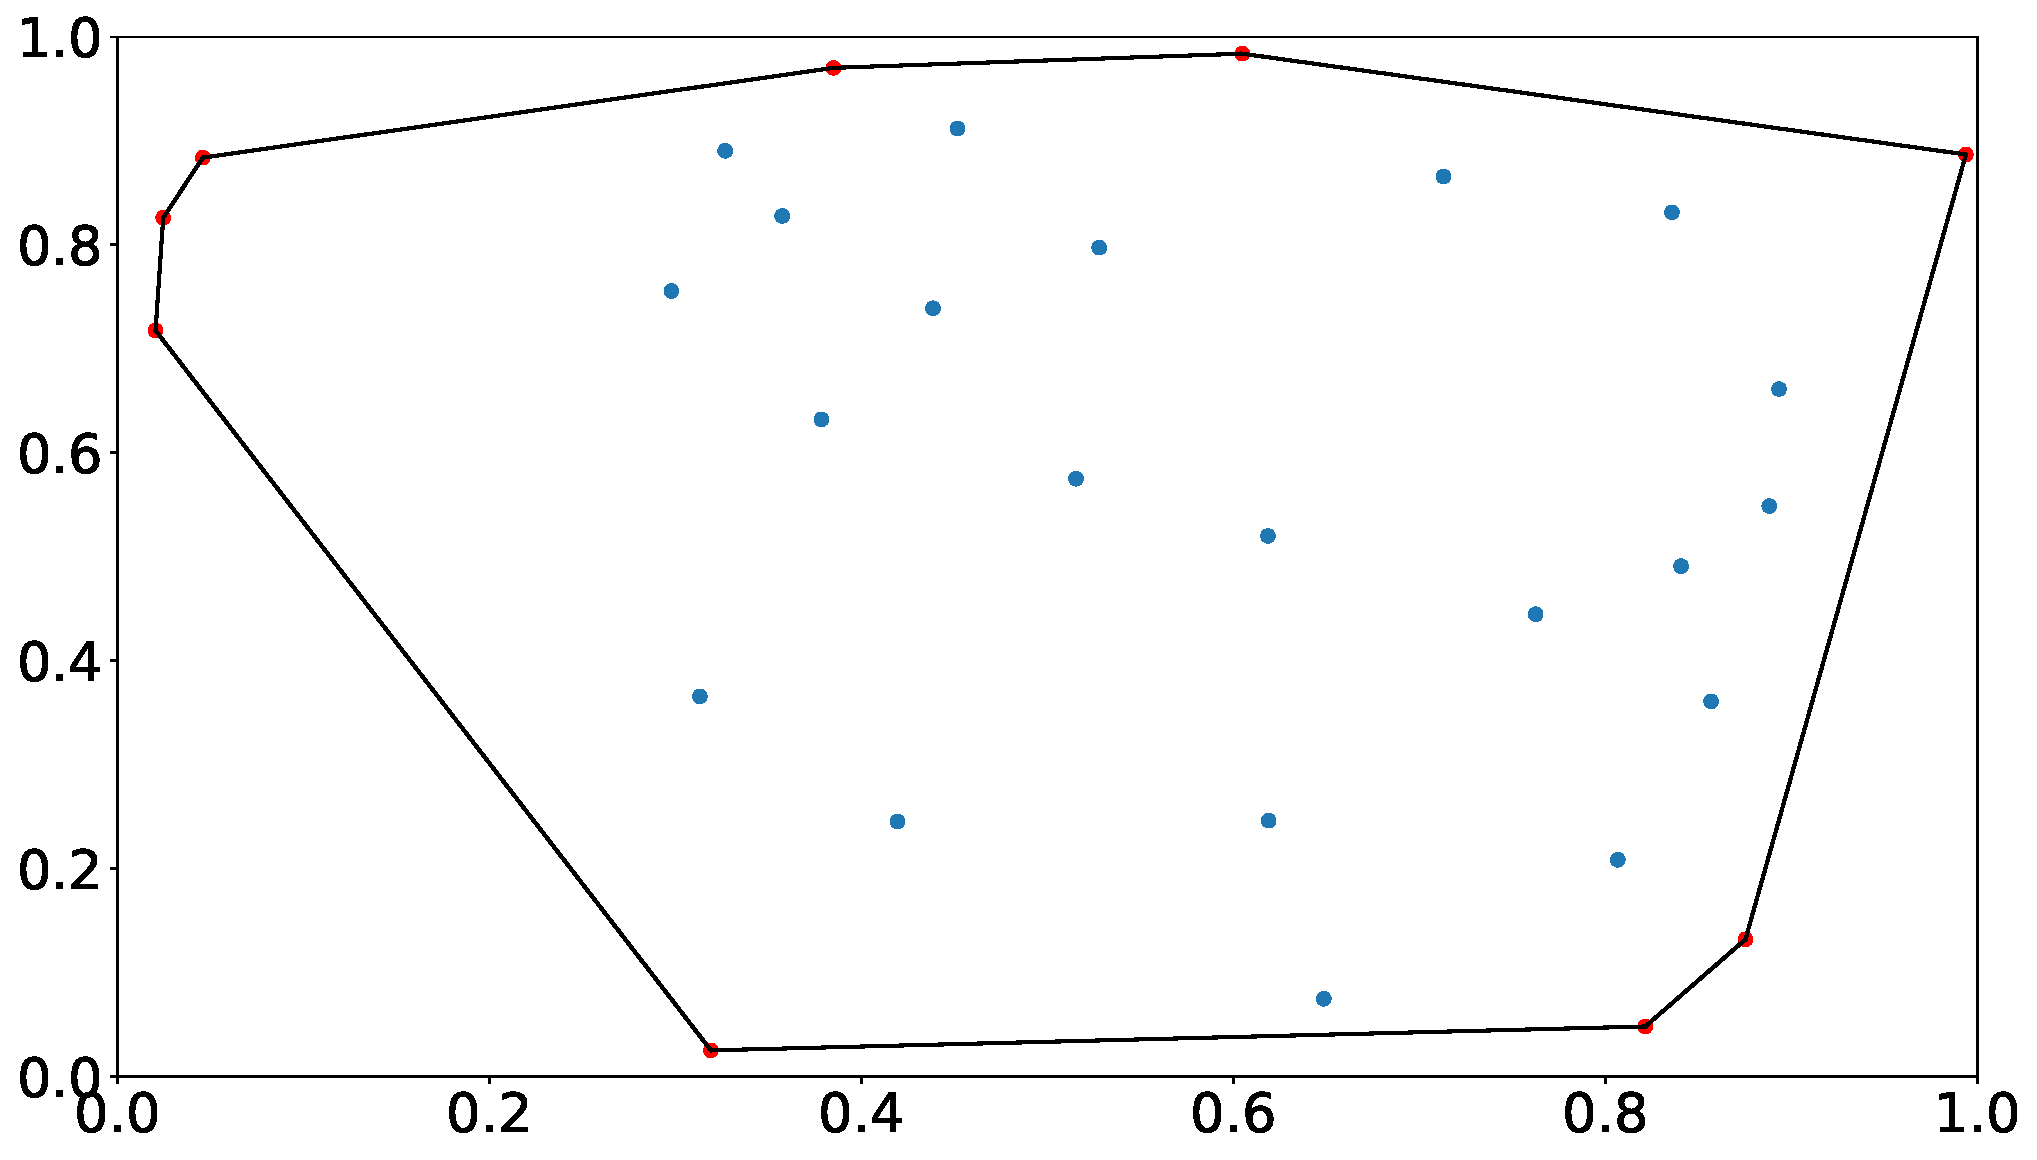
\includegraphics[width=\linewidth]{imgs/v-rep}
  \caption{Visualization of the V-representation of a set}%
  \label{fig:v-rep-example}
\end{figure}

A more useful representation of such regions is the \enquote{H-representation}.
In such a representation, the intersection of a finite number of half-spaces
describes the region. A half-space is one of the two parts in which a
hyper-plane divides an affine space. Since half-spaces are linear inequalities,
the H-representation becomes the matrix inequality
%
\begin{equation}
  Ax\leq{}b,
\end{equation}
%
where \(A\) is a matrix of coefficients, \(x\) is a point in space and \(b\) is
a vector of real numbers. The number of rows in \(A\) and \(b\) is the same as
the number of half-spaces defining the region. All points satisfying the
inequality are inside the region, making it easy to test set membership.
Figure~\ref{fig:h-rep-example} shows the half-spaces that compose the
H-representation of the same convex polytope presented in
Figure~\ref{fig:v-rep-example}. Equation~\ref{eq:h-rep-example} shows the
inequation that describes the region. The selected side is not shown for each
half-space but is the one in which intersections with the other selected halves
make the convex region in the middle.

\begin{equation}
  \label{eq:h-rep-example}
  \begin{bmatrix}
    -0.91 & -0.39 \\
    0.04  & -0.99 \\
    0.98  & -0.15 \\
    0.84  & -0.54 \\
    -0.24 & 0.96  \\
    0.24  & 0.97  \\
    -0.06 & 0.99  \\
    -0.99 & 0.03  \\
    -0.93 & 0.34
  \end{bmatrix}x \leq
  \begin{bmatrix}
    -0.30 \\
    -0.01 \\
    0.84  \\
    0.66  \\
    0.84  \\
    1.10  \\
    0.94  \\
    0.00  \\
    0.26
  \end{bmatrix}
\end{equation}

\begin{figure}[!htb]
  \centering
  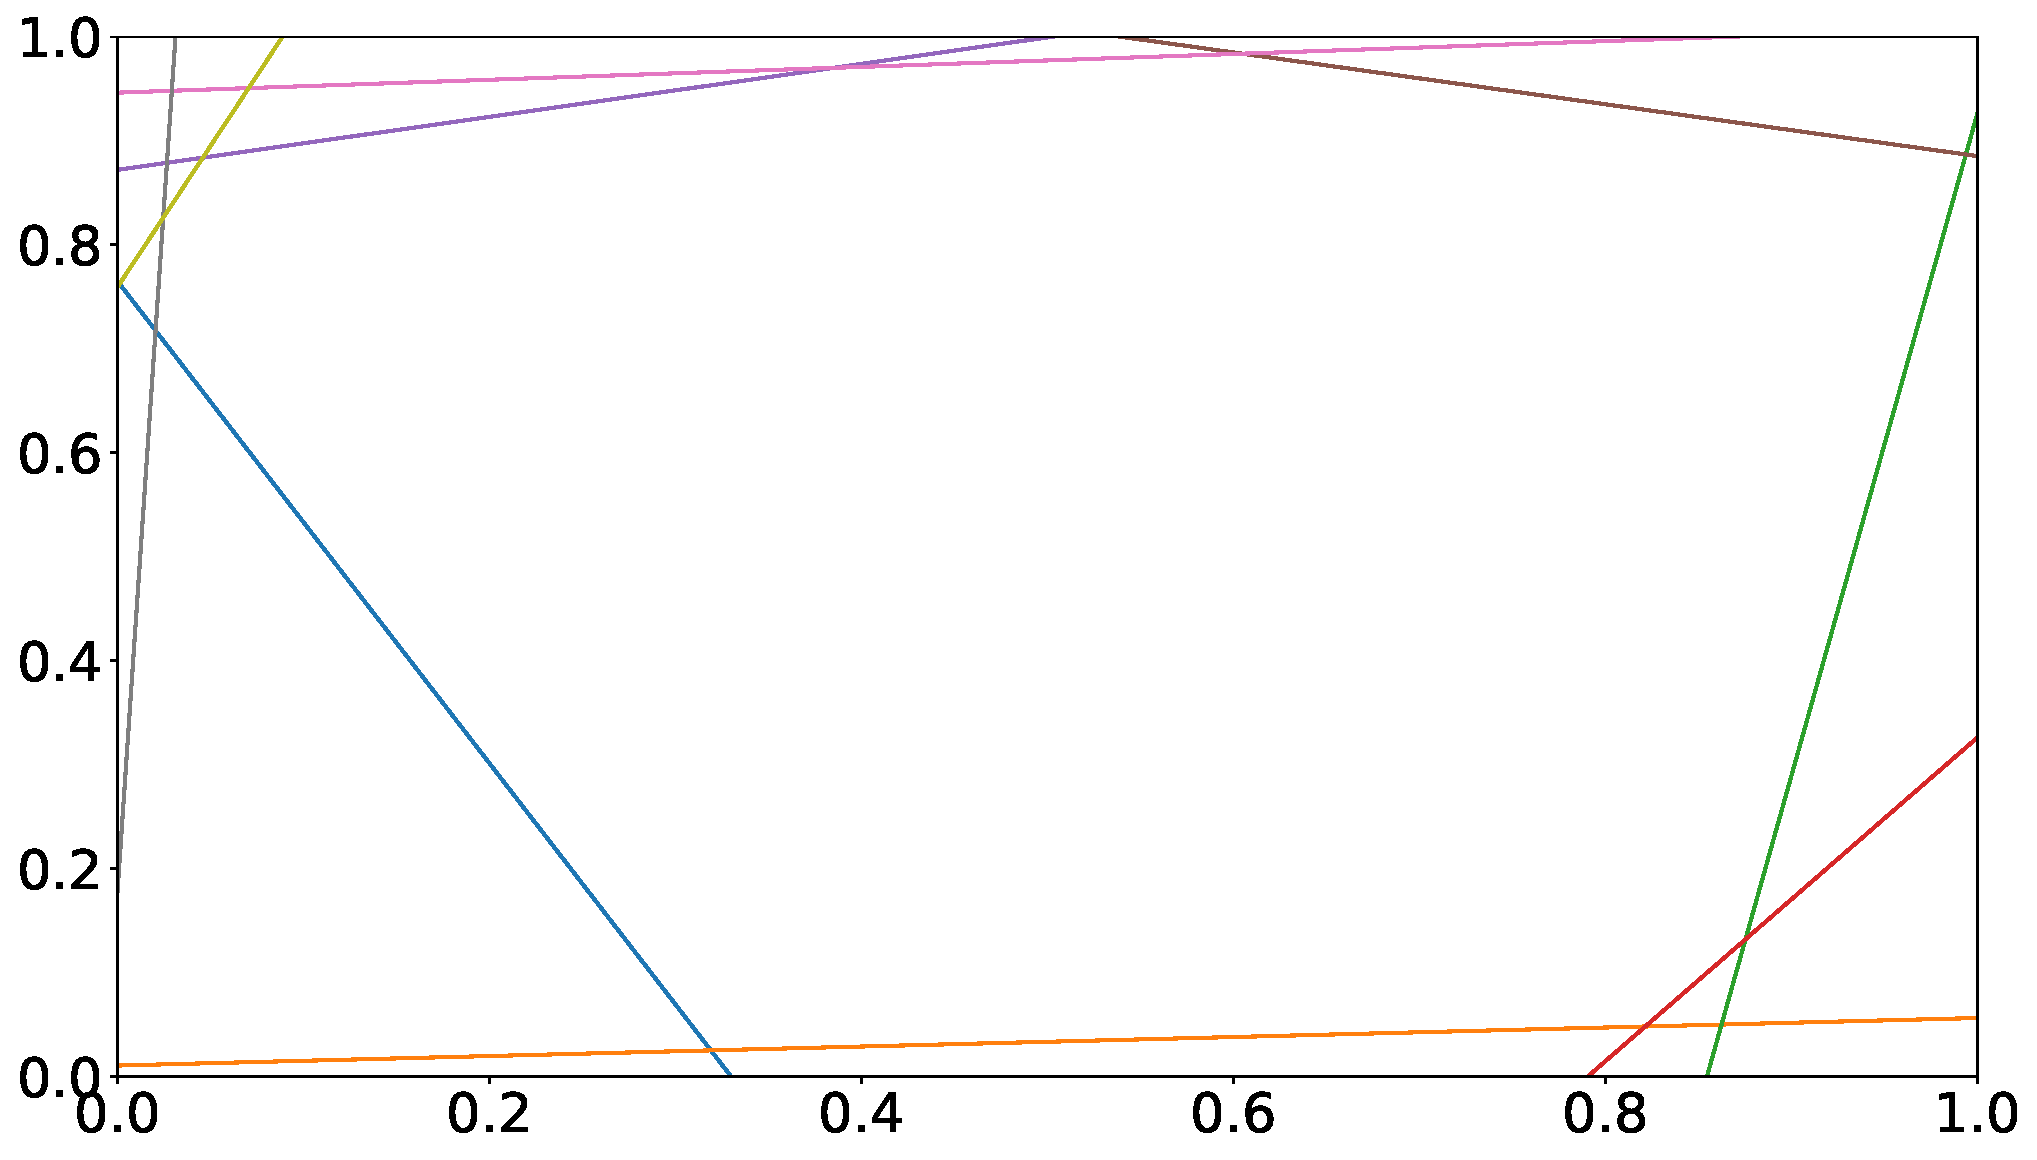
\includegraphics[width=\linewidth]{imgs/h-rep}
  \caption{Visualization of the H-representation of a set}%
  \label{fig:h-rep-example}
\end{figure}

Given a generic shape, it is easy to sample points and build a V-representation
of the polytope, however we need the H-representation to easily test for set
membership. Therefore, we need a way from transforming the V-representation into
the H-representation. Unfortunately, this is not straightforward, but some
algorithms allow us to enumerate the facets given the vertices. Some problems of
such algorithms are the time needed to find the facets of many vertices and how
to find facets in higher-order spaces. However, good algorithms can be used for
the conversion, especially if the computation is done offline, not presenting a
time limitation to the
computation~\parencite{avis.bremner.ea:how,graham.frances-yao:finding,lee:on,mccallum.avis:linear}.

Particular regions can be easily described in a way that it is easy to include
in optimization problems. The ellipsoid is one such region, as it is described
as \(x^{\top}Px\leq{}1\) so that any point \(x\) that satisfies the inequality is
inside the region. Any region described by polynomials can be expressed in a
matrix form and can quickly test membership. Such regions should use their
inequation directly instead of a polytope approximation. We do that to the
Region of Attraction, and it is how we implemented the check to verify if the
state is inside it.

\subsection{Internal Models}%
\label{subsec:internal-models}

To switch modes and controllers of a system the way we propose, one must pay
attention to the controller's internal states and the control signal's
continuity. Also, since every \CG{} unit has its controller and model, the
destination \CG{} must be updated to a valid state before switching. There are
many ways to do so, and we will present some.

One way is to run all \CG{}s in parallel. The optimization problem of the
inactive units does not need to run with complete constraints. It can be relaxed
only to contain the region constraint on the virtual reference; also, the
observer can be ignored. It is necessary to find the virtual reference, which
will be close to the constraint region's border, which is closest to the real
system's state. Notice that, in this case, we are not looking for a virtual
reference closest to the real reference but to the real system's state. By doing
so, the internal model's and the controller's states will always be valid.

However, this approach can be resource-intensive, as it still computes the
optimization problem at every sample. It is also possible to run the observer
and update the internal model's states without checking for constraint
violations, but this does not solve the controller's state problem. Another
technique needs to be combined to find them.

Another way of guaranteeing valid states is to compute the states before
changing mode. Two ways of computing the states are: by inverting the system and
controller equations and by simulation. The first approach has a very low
computational resource impact but may not be possible or yield approximations
due to uncertainties. For systems with integrators, for example, there will be
infinitely many results. Another problem is that even though the system has only
one steady-state solution, it can have many transient ones.

The simulation becomes interesting, even though it is more computationally
intensive, as it can calculate a state that better matches the current
transitory characteristics of the real system. It can also find the model's and
controller's states at once, guaranteeing that there is no mismatch. To use the
simulation approach, execute the simulation right before changing modes, using
the internal controller and model, and setting the reference to the real
system's current state. This yields a valid steady-state model's and
controller's state. However, this technique does not guarantee control signal
continuity (which might even be impossible on some systems) without adjustments.

\subsection{Region of Attraction Estimation}%
\label{subsec:roa-estimation}

The Lyapunov approach presented in Section~\ref{sec:region-of-attraction} can
easily estimate the region of attraction. The presented approach makes use of a
quadratic Lyapunov candidate, but it is not necessary, as it is possible to find
functions of any form. The function should easily check if a point belongs to
the region, as it will be done frequently. Quadratic forms, such as the simple
one presented or those generated by Sum Of Squares techniques, are recommended
since they can easily and computationally inexpensively check set membership.

The region of attraction needs to be larger than the constraints region and
needs to intersect all mode's regions of attraction to and from which it can
switch. Because of this, it is necessary to guarantee the intersection. However,
LMIs usually try to optimize the size of the region of attraction by making it
as big as possible or as small as possible. Since the exponential stability
tries to minimize the size of the region of attraction, we need a way to ensure
a minimum region size.

Consider the region of attraction described by
%
\begin{equation}
  x^{\top}Px \le{} 1,
\end{equation}
%
where \(x\) is the point that should be inside the region of attraction. Note
that, numerically, a number smaller than \(1\) may be necessary to make the
problem feasible.

If the LMI is written in terms of \(P\), it can be used directly to force the
region to be big enough to contain the point \(x\). If the LMI is written in
terms of \(P^{-1}\), simply applying Schur's complement yields a valid LMI:
%
\begin{equation}
  \label{eq:lmi-point-inside-roa}
  \begin{bmatrix}
    P^{-1}   & x \\
    x^{\top} & 1
  \end{bmatrix} \succ \mathbf{0},
\end{equation}

You need to add one of such LMIs to your optimization problem for each mode that
is allowed to switch from or to the current mode. The point \(x\) does not need
to be the same for two modes that intersect, as placing the points some distance
apart creates a larger region of intersection, which gives a margin for errors.

To illustrate the choice of \(x\), consider the switched system composed of
three modes shown in Figure~\ref{fig:choice-x-roa-diff}. The stars represent
each mode's linearization point, the filled ellipses its constraints regions,
the unfilled circles the regions of attractions and the black dots the points
used in the LMIs to ensure the RoA's size. Note the intersection region formed
in the middle, displayed in yellow.

Now compare it with the same system, but only one point used for all systems,
depicted in Figure~\ref{fig:choice-x-roa-same}. See how smaller is the
intersection of regions of attraction and constraints (in yellow). The proposed
technique will be much more efficient in the first case, since it will result in
an earlier switch.

\begin{figure}[!htb]
  \centering
  \begin{subfigure}[b]{.45\linewidth}
    \centering
    \includesvg[width=\linewidth]{imgs/roa-choice-of-x-diff.svg}
    \caption{Choosing different \(x\) for each RoA}%
    \label{fig:choice-x-roa-diff}
  \end{subfigure}
  %
  \begin{subfigure}[b]{.45\linewidth}
    \centering
    \includesvg[width=\linewidth]{imgs/roa-choice-of-x-same.svg}
    \caption{Choosing the same \(x\) for all RoA}%
    \label{fig:choice-x-roa-same}
  \end{subfigure}
  \caption{Different RoA's intesections}%
  \label{fig:choices-of-x}
\end{figure}
